% ---------------------------------------------------
\chapter{FLCR Compiler}
\label{chap:flcr-compiler}
% ---------------------------------------------------

% Toggle for showing the LLVM Pass section (change to \showflcrpassfalse to hide)
\newif\ifshowflcrpass
\showflcrpasstrue

\section*{Overview}
This chapter details the implementation of Function-Level Code Replication (FLCR)
within the compiler framework. The transformation is organized into eight
phases (A–H), followed by runtime initialization of the Replica Selector Table (RST).
Each phase represents a distinct compiler pass responsible for outlining, cloning,
instrumentation, and metadata emission to enable self-validating replicated code.

% ---------------------------------------------------
% ---------------------------------------------------
\section*{Tool Flow}
Figure~\ref{fig:flcr-tool-flow} shows the complete FLCR build pipeline,
from protected source code to a post-linked binary with injected metadata.
This process is designed to integrate cleanly with any LLVM-based toolchain
and uses standard intermediate formats for compatibility with both Clang
and external linkers.

\begin{figure}[t]
  \centering
  % Update to your actual path if needed
  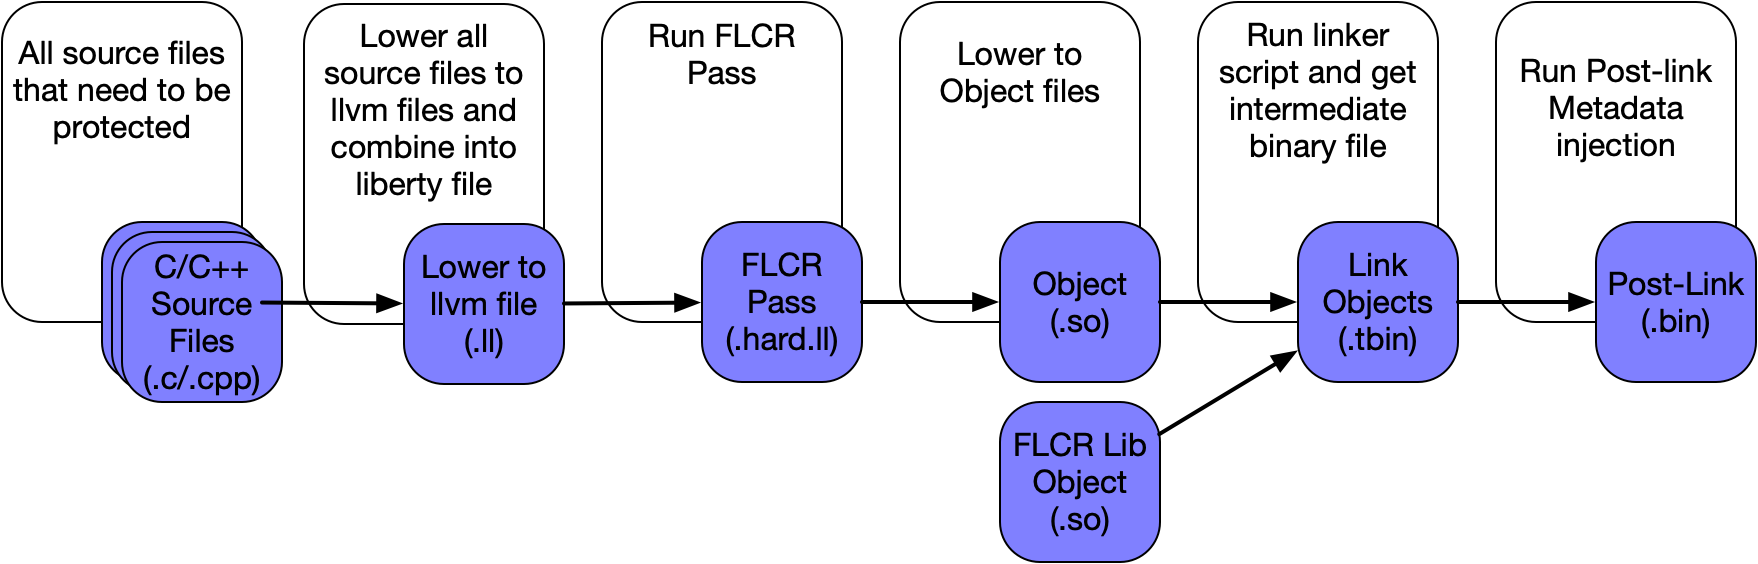
\includegraphics[width=\linewidth]{Chapter-10/figs/flcr-tool-flow.png}
  \caption{FLCR compiler and tool flow. Protected sources are lowered to LLVM IR,
           transformed by the FLCR pass, compiled to objects, linked with the FLCR
           runtime library, and finalized through post-link metadata injection.}
  \label{fig:flcr-tool-flow}
\end{figure}

\paragraph{Stages (left to right).}
\begin{enumerate}
  \item \textbf{Source Collection.}  
        Identify and gather all C/C++ source files that must be protected under FLCR.
        These files form the logical protection unit for the build.
  \item \textbf{IR Generation and Bundling.}  
        Each source is lowered to LLVM IR (\texttt{.ll}) using the standard front end.
        All IR units are then combined into a single IR “library” module for pass execution.
  \item \textbf{Run FLCR Pass.}  
        The FLCR compiler pass transforms the combined IR to insert validation metadata,
        redirection logic, and function clones, producing a hardened module
        (\texttt{.hard.ll}).
  \item \textbf{Lower to Object Files.}  
        The transformed IR is compiled to native object files (\texttt{.o}/\texttt{.so}).
        The FLCR runtime support library is built at this stage as a companion object.
  \item \textbf{Linking.}  
        Application and runtime objects are linked using the standard linker script
        to generate an intermediate binary (\texttt{.tbin}). This step merges all
        function tables and ensures consistent section layout.
  \item \textbf{Post-Link Metadata Injection.}  
        The post-link tool scans the intermediate binary, computes function sizes and
        checksums, and populates the lookup tables emitted by the FLCR pass.
        The final binary (\texttt{.bin}) is fully self-validating.
\end{enumerate}


\paragraph{Artifacts.}
\begin{itemize}
  \item \texttt{*.ll} — per-source LLVM IR files combined into a single library.
  \item \texttt{*.hard.ll} — IR after FLCR pass; includes cloned variants and metadata.
  \item \texttt{*.o}, \texttt{*.so} — compiled objects, including the FLCR runtime object.
  \item \texttt{*.tbin} — intermediate binary prior to metadata injection.
  \item \texttt{*.bin} — final FLCR-protected executable with populated lookup tables.
\end{itemize}


% ---------------------------------------------------
\ifshowflcrpass
  % ---------------------------------------------------
\section*{LLVM Pass}
FLCR is realized as a fixed sequence of compiler passes (A–H). Each pass consumes
IR and/or metadata from the previous step and produces artifacts that the next step
relies on. The table summarizes each phase.

\begin{table}[t]
  \centering
  \renewcommand{\arraystretch}{1.15}
  \begin{tabularx}{\linewidth}{|c|X|X|X|}
    \hline
    \textbf{Phase} & \textbf{Purpose} & \textbf{Key Operations} & \textbf{Primary Outputs} \\ \hline
    A & Entry wrapping & Outline original entry; insert \texttt{code\_init()} and tail-call & New entry thunk; \texttt{.outlined} body \\ \hline
    B & Candidate selection & Apply include/exclude; filter intrinsics/decls; stable order & \textit{Bases}, \textit{BaseIndex} \\ \hline
    C & Indirect resolver & Interpose on function-pointer calls via \texttt{resolve()} & Indirect callsites become resolvable \\ \hline
    D & Clone stubs & Declare \(N\) variants per base (sig/attrs preserved) & \textit{ClonesMap} (stubs) \\ \hline
    E & Globals/metadata & Define lookup, checksums, sizes; set sections; keep alive & \texttt{func\_lookup}, \texttt{func\_checksum}, \texttt{func\_size} \\ \hline
    F & Direct-call rewrite & Replace direct calls to bases with loads from lookup slot & Calls to candidates go via \texttt{func\_lookup[idx]} \\ \hline
    G & Deep clone bodies & Clone base body into each stub; remap SSA & Materialized variant bodies \\ \hline
    H & Catalog/finalize & Build RO address array; optionally drop/keep bases & \texttt{func\_array}; cleaned module \\ \hline
    Runtime & Initialize RST & Validate variants; select first valid; write lookup slot & Populated \texttt{func\_lookup} \\ \hline
  \end{tabularx}
  \caption{Phase purposes, operations, and outputs for the FLCR pass pipeline.}
  \label{tab:flcr-pass-layout}
\end{table}

\clearpage
\subsection*{Phase A — Runtime Initialization Wrapper}
This phase wraps the program’s entry point to integrate the runtime initialization sequence
before any \textbf{hardened user code} executes.
The compiler locates the configured entry function (typically \texttt{main} or another designated symbol)
and outlines its body into a secondary function suffixed with \texttt{.outlined}.
The original entry is reconstructed to first invoke \texttt{code\_init()}—the runtime routine responsible
for preparing FLCR metadata, global tables, and replica structures—before transferring control
to the outlined body.
This guarantees that all fault-tolerance metadata is initialized prior to entering hardened user code,
ensuring that subsequent phases of replication and validation operate on a consistent runtime state.
The outlined entry function is marked for exclusion from later replication stages to avoid
recursive transformation of the bootstrap logic itself.

\begin{algorithm}[H]
\caption{Phase A — Outline Entry and Inject Initialization}
\label{alg:phaseA}
\begin{algorithmic}[1]
\State \textbf{Input:} Module \textit{M}, CONFIG \textit{C}
\State Entry $\gets$ M.\textproc{getFunction}(C.ENTRY)
\If{Entry = null \textbf{ or } Entry.\textproc{isDeclaration}()} \State \Return \EndIf
\State Outlined $\gets$ \textproc{clone\_signature}(Entry, name = Entry.name + ``.outlined'')
\State \textproc{move\_all\_blocks}(Entry $\rightarrow$ Outlined)
\State \textbf{rebuild\_body}(Entry):
\State \hspace{\algorithmicindent}\textproc{call} \texttt{code\_init}()
\State \hspace{\algorithmicindent}\textproc{ret call} Outlined(original\_args)
\State \textproc{mark\_for\_exclusion}(Entry)
\end{algorithmic}
\end{algorithm}
\clearpage

% ---------------------------------------------------
\subsection*{Phase B — Hardened Function Selection}
This phase assigns each hardened function a \textbf{global group index}
that identifies the function and all of its replicated variants across the FLCR system.
Every runtime table—such as the \textbf{Indirect Table (ITab)}, checksum table,
size table, and function lookup array—is organized in contiguous blocks per group,
allowing all replicas of a given function to be addressed relative to their shared index.

For each function group, the compiler generates \(N\) replicas.
Each replica’s \textbf{unique index} is derived as:
\[
\text{UniqueIndex} = \text{GroupIndex} \times N + \text{ReplicaID}
\]
where \textit{GroupIndex} identifies the function family,
and \textit{ReplicaID} enumerates the variants within that group.

Candidate selection is driven by user configuration, allowing selective hardening of key routines.
Two mutually exclusive mechanisms are supported:
an \textbf{inclusion list}, which explicitly enumerates functions to replicate,
or an \textbf{exclusion list}, which omits specified routines while including all others.
Intrinsic functions, declarations without bodies, and any preexisting tolerance variants
are automatically excluded.

Each remaining function becomes a \textbf{base function} and receives a stable global group index.
Sorting by name ensures deterministic ordering, preserving identical indices across builds
and toolchains, independent of link order or optimization variance.

The result of this phase is a reproducible mapping from
\textbf{group ID → base function address} and a derived formula for computing
each replica’s unique index, forming the structural foundation of all FLCR metadata tables.

\begin{algorithm}[H]
\caption{Phase B — Collect Base Functions}
\label{alg:phaseB}
\begin{algorithmic}[1]
\State \textbf{Input:} Module \textit{M}, CONFIG \textit{C}
\State IncludeSet $\gets$ parse\_csv(C.INCLUDE\_CSV)
\State ExcludeSet $\gets$ parse\_csv(C.EXCLUDE\_CSV) $\cup$ \{C.ENTRY\}
\State UseInclude $\gets$ (IncludeSet $\neq \emptyset$)
\State Bases $\gets$ [\,]
\For{each Function F in M}
  \If{F.\textproc{isDeclaration}() \textbf{ or } \textproc{is\_intrinsic}(F) \textbf{ or } \textproc{name\_contains}(F, ``\_tolerance\_'')} \State \textbf{continue} \EndIf
  \If{UseInclude \textbf{ and } F.name $\notin$ IncludeSet} \State \textbf{continue} \EndIf
  \If{$\neg$UseInclude \textbf{ and } F.name $\in$ ExcludeSet} \State \textbf{continue} \EndIf
  \State Bases.push(F)
\EndFor
\State \textproc{sort}(Bases by F.name ascending)
\For{each (i, B) in \textproc{enumerate}(Bases)} \State BaseIndex[B] $\gets$ i \EndFor
\end{algorithmic}
\end{algorithm}
\clearpage

% ---------------------------------------------------
\subsection*{Phase C — Runtime Resolver Injection}
This phase locates all \textbf{indirect call sites}—calls whose targets are not
statically known at compile time. These include function pointer calls, callbacks,
and dynamically computed destinations.

Each indirect call is rewritten to pass through the runtime \texttt{resolve()}
routine, which searches the \textbf{Indirection Map (IMap)} to obtain the hardened
function address associated with the original pointer.

\begin{center}
\texttt{call *ptr(args)} 
$\quad\Rightarrow\quad$
\texttt{target = resolve(ptr)} \\
\texttt{call target(args)}
\end{center}

This transformation ensures that all dynamically dispatched calls
are redirected through the IMap, establishing a uniform runtime lookup
for indirect control transfers.

\begin{algorithm}[H]
\caption{Phase C — Rewrite Indirect Calls}
\label{alg:phaseC}
\begin{algorithmic}[1]
\State \textbf{Input:} Module \textit{M}
\For{each Function F in M}
  \For{each CallSite CS in F}
    \If{CS.\textproc{isDirect}()} \State \textbf{continue} \EndIf
    \State callee\_ptr   $\gets$ CS.\textproc{getCalleeOperand}()
    \State callee\_i8ptr $\gets$ \textproc{bitcast}(callee\_ptr $\rightarrow$ i8*)
    \State resolved\_i8ptr $\gets$ \textproc{call}~i8*~\texttt{resolve}(callee\_i8ptr)
    \State resolved\_typed $\gets$ \textproc{bitcast}(resolved\_i8ptr $\rightarrow$ \textproc{type}(callee\_ptr))
    \State CS.\textproc{setCallee}(resolved\_typed)
  \EndFor
\EndFor
\end{algorithmic}
\end{algorithm}
\clearpage

% ---------------------------------------------------
\subsection*{Phase D — Hardened Replica Declaration}
In this phase, the compiler declares empty placeholder functions representing
the replicated variants of each hardened function selected in the previous phase.
These declarations create a structural template for every function group, but
no executable body is yet assigned.

For each base function \(B_i\), a total of \(N\) hardened variants are declared:
the original function corresponds to variant 0, and the remaining \(N{-}1\)
variants are uniquely named derivatives. All replicas preserve the base
function’s signature, attributes, and calling conventions to ensure drop-in
interchangeability during later phases.

Each declared replica is recorded in the \textbf{Clone Map}, which associates
the base function with its corresponding set of variants. These stubs form
the foundation for later cloning and section placement, enabling subsequent
phases to materialize their bodies, assign fault-tolerant sections, and
finalize linkage.

\begin{center}
\textit{Example:} \\
\texttt{foo} $\rightarrow$ 
\{\texttt{foo\_tolerance\_1}, \texttt{foo\_tolerance\_2}, \ldots, \texttt{foo\_tolerance\_(\(N{-}1\))}\}
\end{center}

At this stage, only the declarations are emitted—no bodies or control-flow
graphs exist yet. The hardened replica declarations ensure that symbol
visibility and linkage metadata are available to subsequent transformation
passes.

\begin{algorithm}[H]
\caption{Phase D — Create Empty Clone Stubs}
\label{alg:phaseD}
\begin{algorithmic}[1]
\State \textbf{Input:} Module \textit{M}, CONFIG \textit{C}
\For{each base B in Bases}
  \State ClonesMap[B] $\gets$ [\,]
  \For{$j$ in [0..C.N-1]}
    \State name $\gets$ B.name + ``\_tolerance\_'' + \textproc{itoa}(j)
    \State Stub $\gets$ \textproc{declare\_function\_like}(B, name, external\_linkage)
    \State \textproc{copy\_attributes}(Stub, from = B)
    \If{C.SEC\_CLONES \text{ not empty}} \State \textproc{set\_section}(Stub, C.SEC\_CLONES) \EndIf
    \State ClonesMap[B].append(Stub)
  \EndFor
\EndFor
\end{algorithmic}
\end{algorithm}
\clearpage

% ---------------------------------------------------
\subsection*{Phase E — Global Metadata Emission}
This phase defines the global data structures that describe the replicated
functions and their runtime properties. These structures are emitted as
compiler-generated globals and linked directly with the hardened program image.

Three primary tables are created:

\begin{itemize}
  \item \textbf{Function Address Table (\texttt{func\_lookup})} — a writable
  array of pointers, one per hardened function group. At runtime, each entry
  will be updated with the address of the first validated replica.
  \item \textbf{Function Hash Table (\texttt{func\_hash})} — stores integrity
  digests for all variants. Each hash corresponds to the verified contents of
  the replicated function’s text region.
  \item \textbf{Function Size Table (\texttt{func\_size})} — records the byte
  length of every variant body, used during hashing and runtime validation.
\end{itemize}

The tables are dimensioned according to the total number of function groups and
the replication count:
\[
\text{Total Entries} = |Bases| \times N
\]
All tables are emitted as writable globals, optionally placed into target-specific
sections (e.g., \texttt{.lookup}, \texttt{.meta}) as defined by the build
configuration. Each global is marked as \texttt{compiler\_used} to ensure
preservation through link-time optimization.

Together, these tables form the structural metadata interface between the
compiler-generated replicas and the runtime repair subsystem, providing the
necessary mapping and validation data for dynamic fault recovery.

\begin{algorithm}[H]
\caption{Phase E — Emit Global Metadata Structures}
\label{alg:phaseE}
\begin{algorithmic}[1]
\State \textbf{Input:} Module \textit{M}, CONFIG \textit{C}
\State NumBases $\gets$ \textproc{size}(Bases)
\State Total $\gets$ NumBases $\times$ C.N
\State LookupGV   $\gets$ \textproc{define\_global}(``func\_lookup'',  array[NumBases] of i8*, writable)
\State ChecksumGV $\gets$ \textproc{define\_global}(``func\_checksum'', array[Total] of u32, writable)
\State SizeGV     $\gets$ \textproc{define\_global}(``func\_size'',     array[Total] of u32, writable)
\If{C.SEC\_LOOKUP \text{ not empty}}
  \State \textproc{set\_section}(LookupGV,   C.SEC\_LOOKUP)
  \State \textproc{set\_section}(ChecksumGV, C.SEC\_LOOKUP)
  \State \textproc{set\_section}(SizeGV,     C.SEC\_LOOKUP)
\EndIf
\State \textproc{mark\_compiler\_used}([LookupGV, ChecksumGV, SizeGV])
\end{algorithmic}
\end{algorithm}
\clearpage

% ---------------------------------------------------
\subsection*{Phase F — Direct Call Rewrite}
This phase modifies all \textbf{direct} call instructions that target hardened
functions, ensuring that they too are routed through the \textbf{Indirect Table
(ITab)}. Indirect calls were already redirected in Phase C; this step brings
direct calls into the same runtime-controlled indirection path.

For each direct call, the compiler replaces the callee operand with a pointer
loaded from the ITab at the function’s assigned group index. This ensures that
both direct and indirect calls uniformly reference replicas through the same
runtime-managed lookup structure.

\begin{center}
\textit{Example Transformation:}
\end{center}

\begin{verbatim}
Original:
    call void @foo()
Transformed:
    %ptr = load i8*, &ITab[GroupID]
    %callee = bitcast i8* %ptr to void ()*
    call void %callee()
\end{verbatim}

After runtime initialization, each ITab entry contains the validated address of
a replica chosen from the Function Address Table. As a result, all calls—whether
originally direct or indirect—are transparently dispatched to fault-free
replicas without compiler or linker intervention.

\begin{algorithm}[H]
\caption{Phase F — Rewrite Direct Calls via Lookup Table}
\label{alg:phaseF}
\begin{algorithmic}[1]
\State \textbf{Input:} Module \textit{M}, LookupGV
\For{each Function F in M}
  \For{each CallSite CS in F}
    \State Callee $\gets$ CS.\textproc{getDirectCallee}()
    \If{Callee = null \textbf{ or } Callee $\notin$ BaseIndex} \State \textbf{continue} \EndIf
    \State idx $\gets$ BaseIndex[Callee]
    \State slot\_ptr $\gets$ \textproc{gep}(LookupGV, [0, idx]) \Comment{\&func\_lookup[idx]}
    \State raw\_i8 $\gets$ \textproc{volatile\_load}(slot\_ptr, align=8)
    \State typed\_ptr $\gets$ \textproc{bitcast}(raw\_i8 $\rightarrow$ \textproc{type}(Callee))
    \State CS.\textproc{setCallee}(typed\_ptr)
  \EndFor
\EndFor
\end{algorithmic}
\end{algorithm}
\clearpage

% ---------------------------------------------------
\subsection*{Phase G — Clone Variant Bodies}
This phase materializes the replicated bodies of all hardened functions.  
For each base function selected in Phase B, \(N-1\) additional variants are created,
each containing a deep copy of the original function’s body, preserving
instruction semantics, control flow, and data dependencies.

Each clone is assigned a unique identifier derived from its group index and
replica number. This identifier is used to tag the variant as part of a hardened
function group and to establish its fixed position within the
\textbf{Function Address Table}.  
The cloning process remaps SSA values, updates references to local symbols, and
copies all attributes and calling conventions from the base function.

\begin{center}
\textit{Example Transformation:}
\end{center}

\begin{verbatim}
Original:
    define void @foo() { ... }

After cloning (N = 3):
    define void @foo_tolerance_0() { ... }
    define void @foo_tolerance_1() { ... }
    define void @foo_tolerance_2() { ... }
\end{verbatim}

These cloned variants are not immediately active but are referenced indirectly
through the ITab once the Replica Selector Table is initialized at runtime.
This ensures that all hardened functions have a complete set of executable
replicas ready for validation and substitution.

\begin{algorithm}[H]
\caption{Phase G — Deep Clone Variant Bodies}
\label{alg:phaseG}
\begin{algorithmic}[1]
\For{each base B in Bases}
  \For{$j$ in [0..C.N-1]}
    \State Dst  $\gets$ ClonesMap[B][j]
    \State VMap $\gets$ \textproc{map}\{\}
    \State \textproc{map\_formals}(B.args $\rightarrow$ Dst.args, into = VMap)
    \State \textproc{clone\_body}(src = B, dst = Dst, value\_map = VMap)
    \If{C.SEC\_CLONES \text{ not empty}} \State \textproc{set\_section}(Dst, C.SEC\_CLONES) \EndIf
  \EndFor
\EndFor
\end{algorithmic}
\end{algorithm}
\clearpage

% ---------------------------------------------------
\subsection*{Phase H — Catalog and Finalize}
The final compile-time phase assembles the complete catalog of all hardened functions
and their replicas. It consolidates metadata generated in earlier phases and assigns
definitive slots within the \textbf{Function Address Table (FAT)},
\textbf{Function Size Table}, and \textbf{Function Hash Table}.

For each hardened function group:
\begin{itemize}
  \item Each replica, including the variant derived from the original function body,
        is assigned a contiguous block of \(N\) entries in the FAT.
  \item Each group begins at the global index established in Phase~B and covers all
        hardened variants associated with that function.
  \item Placeholder entries are emitted for both the Function Size and Hash tables;
        these will be completed later by the post-link tool.
  \item All tables are marked \texttt{compiler\_used} and placed in fixed sections
        to prevent removal or reordering during link-time optimization.
\end{itemize}

After catalog construction, the unreplicated version of each original function is cut,
leaving only hardened variants under compiler control.  
This guarantees that all runtime execution paths pass through the indirection
structures established by the FLCR pipeline.

\begin{center}
\textit{Example Layout (N = 3):}
\end{center}

\begin{verbatim}
Function Address Table (FAT)
 [0] foo_tolerance_0 → <address>
 [1] foo_tolerance_1 → <address>
 [2] foo_tolerance_2 → <address>
 [3] bar_tolerance_0 → <address>
 [4] bar_tolerance_1 → <address>
 [5] bar_tolerance_2 → <address>

Function Size Table
 size: [ -, -, -, -, -, - ]

Function Hash Table
 hash: [ -, -, -, -, -, - ]
\end{verbatim}

The FAT defines the final layout of all hardened replicas but does not yet contain
resolved addresses at compile time.  
Physical addresses are assigned later by the linker when the final binary is produced.  
Subsequently, during the post-link stage, an external tool computes and injects
the corresponding entries for the \textbf{Function Size Table} and
\textbf{Function Hash Table}, completing the metadata set required for runtime
validation and recovery.

\begin{algorithm}[H]
\caption{Phase H — Finalize and Publish Catalog}
\label{alg:phaseH}
\begin{algorithmic}[1]
\State NumBases $\gets$ \textproc{size}(Bases)
\State Total    $\gets$ NumBases $\times$ C.N
\State AllElems $\gets$ array[Total] of i8*
\For{$i$ in [0..NumBases-1]}
  \State Vec $\gets$ ClonesMap[Bases[i]]
  \For{$j$ in [0..C.N-1]}
    \State AllElems[i*C.N + j] $\gets$ \textproc{bitcast\_to\_i8ptr}(Vec[j])
  \EndFor
\EndFor
\State AllGV $\gets$ \textproc{define\_global}(``func\_array'', array[Total] of i8*, init = AllElems, writable = false)
\If{C.SEC\_ALL \text{ not empty}}
  \State \textproc{set\_section}(AllGV, C.SEC\_ALL)
\EndIf
\State \textproc{mark\_compiler\_used}([AllGV])
\For{each base B in Bases}
  \If{C.KEEP\_BASE\_DECLS}
    \State \textproc{delete\_body\_keep\_decl}(B)
  \Else
    \State \textproc{safe\_erase}(B)
  \EndIf
\EndFor
\end{algorithmic}
\end{algorithm}
\clearpage


  \clearpage
\fi
% ---------------------------------------------------
% ---------------------------------------------------
\section*{Runtime FLCR Code}
% ---------------------------------------------------

At runtime, two lightweight routines activate and maintain the replicated code:
\texttt{code\_init()} initializes the metadata tables, and \texttt{resolve()}
handles indirect function lookups. These routines complete the execution model
established by the compiler passes. The initialization phase builds the Indirection
Table (ITab) from validated entries in the Function Address Table (FAT), while the
resolver performs a binary search over the Indirection Map (IMap) to locate the
validated target address for an indirect call.

% ---------------------------------------------------
\subsection*{Metadata Initialization (\texttt{code\_init()})}
\begin{algorithm}[H]
\caption{\texttt{code\_init} — Populate Indirection Table (ITab) from FAT}
\label{alg:code-init-itab}
\begin{algorithmic}[1]
\State \textbf{Inputs:} \texttt{FAT} (Function Address Table), \texttt{FuncSize}, \texttt{FuncHash}, \texttt{NumGroups}, \texttt{N}
\State \textbf{Output:} \texttt{ITab} (Indirection Table)
\For{\texttt{gid} \textbf{in} 0 .. \texttt{NumGroups-1}}
  \For{\texttt{vid} \textbf{in} 0 .. \texttt{N-1}}
    \State \texttt{addr} $\gets$ \texttt{FAT[gid * N + vid]}
    \If{\textproc{validate}(\texttt{addr}, \texttt{FuncSize}, \texttt{FuncHash})}
      \State \texttt{ITab[gid]} $\gets$ \texttt{addr}
      \State \textbf{break}
    \EndIf
  \EndFor
\EndFor
\end{algorithmic}
\end{algorithm}

% ---------------------------------------------------
\subsection*{Resolver (\texttt{resolve()}) — Binary Search over IMap}
\noindent
The resolver performs a \textbf{binary search} within the Indirection Map (IMap),
which stores sorted pairs of \texttt{(orig\_addr, target\_addr)}.  
Given a function pointer, it searches for a matching original address and returns
the validated replica’s address. If no match is found, the resolver returns the
input pointer unchanged, allowing untracked calls to execute normally.

\begin{algorithm}[H]
\caption{\texttt{resolve(ptr)} — Binary search in IMap}
\label{alg:resolve-bsearch}
\begin{algorithmic}[1]
\State \textbf{Input:} \texttt{ptr} (original function pointer), \texttt{IMap} (sorted by \texttt{orig\_addr})
\State \textbf{Output:} \texttt{target} (resolved function pointer)
\State \texttt{key} $\gets$ \textproc{normalize\_ptr}(\texttt{ptr}) \Comment{e.g., cast to \texttt{i8*}}
\State \texttt{lo} $\gets$ 0;\; \texttt{hi} $\gets$ \texttt{IMap.size() - 1}
\While{\texttt{lo} $\le$ \texttt{hi}}
  \State \texttt{mid} $\gets$ (\texttt{lo} + \texttt{hi}) / 2
  \State \texttt{cur} $\gets$ \texttt{IMap[mid].orig\_addr}
  \If{\texttt{key} $==$ \texttt{cur}}
    \State \Return \texttt{IMap[mid].target\_addr}
  \ElsIf{\texttt{key} $<$ \texttt{cur}}
    \State \texttt{hi} $\gets$ \texttt{mid} - 1
  \Else
    \State \texttt{lo} $\gets$ \texttt{mid} + 1
  \EndIf
\EndWhile
\State \Return \texttt{ptr} \Comment{no entry found: return input pointer}
\end{algorithmic}
\end{algorithm}

\section*{Summary}
The FLCR compiler pass pipeline progressively introduces code replication,
metadata emission, and call-site redirection across eight transformation phases.
At runtime, the Replica Selector Table validates each variant and populates
the Function Lookup Table with the first verified address, allowing transparent
execution redirection and robust fault recovery.
